\documentclass{article}
\usepackage{array}
\usepackage[column=0]{cellspace}
\setlength\cellspacetoplimit{6pt}
\setlength\cellspacebottomlimit{6pt}
\usepackage{graphicx} % Required for inserting images
\usepackage{amsmath}
\usepackage{amssymb}
\usepackage{amsthm}
\usepackage{amsfonts}
\usepackage{gensymb}
\newcommand{\myvec}[1]{\ensuremath{\begin{pmatrix}#1\end{pmatrix}}}
\usepackage{graphicx}
\usepackage{mathtools}

\newcommand{\mydet}[1]{\ensuremath{\begin{vmatrix}#1\end{vmatrix}}}
\providecommand{\brak}[1]{\ensuremath{\left(#1\right)}}
\providecommand{\norm}[1]{\left\lVert#1\right\rVert}
\let\vec\mathbf

\title{MathConstruction}

\begin{document}

\section{NCERT 12.10.5.9}

Find the position vector of a point R which divides the line joining two points P and Q whose Position Vectors are $2\vec{a}+\vec{b}$ and $\vec{a}-3\vec{b}$ externally in the ratio $1:2$.Also, Show that P is the mid point of the line segment QR  \\
\textbf{Solution:}
The coordinates and ratio are given in \ref{tab:mytable}
\begin{table}[h]
    \centering
    \begin{tabular}{|c|c|c|}
        \hline
	\textbf{Symbol} & \textbf{Value} & \textbf{Description}\\
        \hline
	$\vec{P}$ & $\myvec{2\\1}$ & Position vector P\\
        \hline
	$\vec{Q}$ & $\myvec{1\\-3}$ & Position vector Q\\
        \hline
	$k$ & $2$ & Ratio\\
        \hline
    \end{tabular}
    \label{tab:mytable}
    \caption{Position vectors P,Q and Ratio K}
\end{table}

Using section formula
\begin{align}
    \vec{R}=\frac{\vec{Q}-k.\vec{P}}{1-k}\\
    \vec{R}=\frac{\myvec{1\\-3}-2\myvec{2\\1}}{1-2}\\
    \vec{R}=\myvec{3\\5}
\end{align}
\begin{table}[h]
    \centering
    \begin{tabular}{|c|c|c|}
        \hline
	\textbf{Symbol} & \textbf{Value} & \textbf{Description} \\
        \hline
	$\vec{R}$ & $\myvec{3\\5}$  & Position vector R\\
        \hline
    \end{tabular}
    \label{tab:mytable}
    \caption{Position vector R}
\end{table}
Position vector R which is a External point
\begin{figure}[!ht]
    \centering
    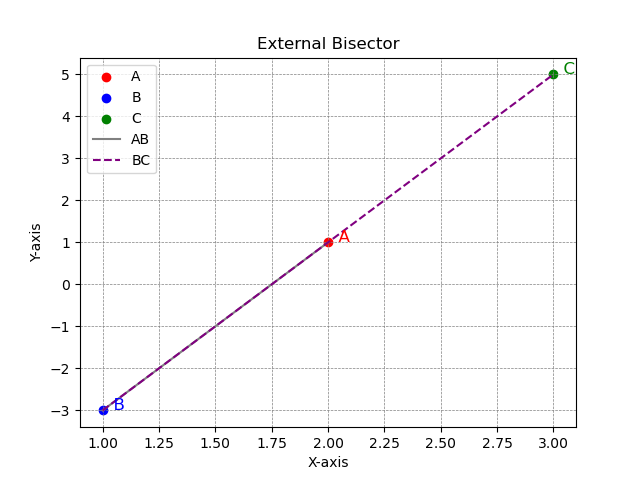
\includegraphics[width=\columnwidth]{/home/ramsai/MathComputing/codes/python/external_bisector.png}
    \caption{point vectors A,B,C}
    \label{fig:enter-label}
\end{figure}
\end{document}
